O grupo 1 da disciplina de Projeto Integrador 1 do segundo semestre de 2015 deverá desenvolver um projeto de balão cativo para monitoramento do estacionamento e das fronteiras do campus da FGA, cujo objetivo é manter um maior controle da movimentação de carros e pessoas nas áreas de alcance do balão, devido os problemas de furtos avaliados anteriormente e, também, devido a possíveis invasões de área.

O estacionamento possui área de 16100 $m^2$, com perímetro de 1215 m. Contudo, a área é extensa e existem locais de estacionamento isolados [figura \ref{img:fga2}].

\begin{figure}[H]
  \centering
  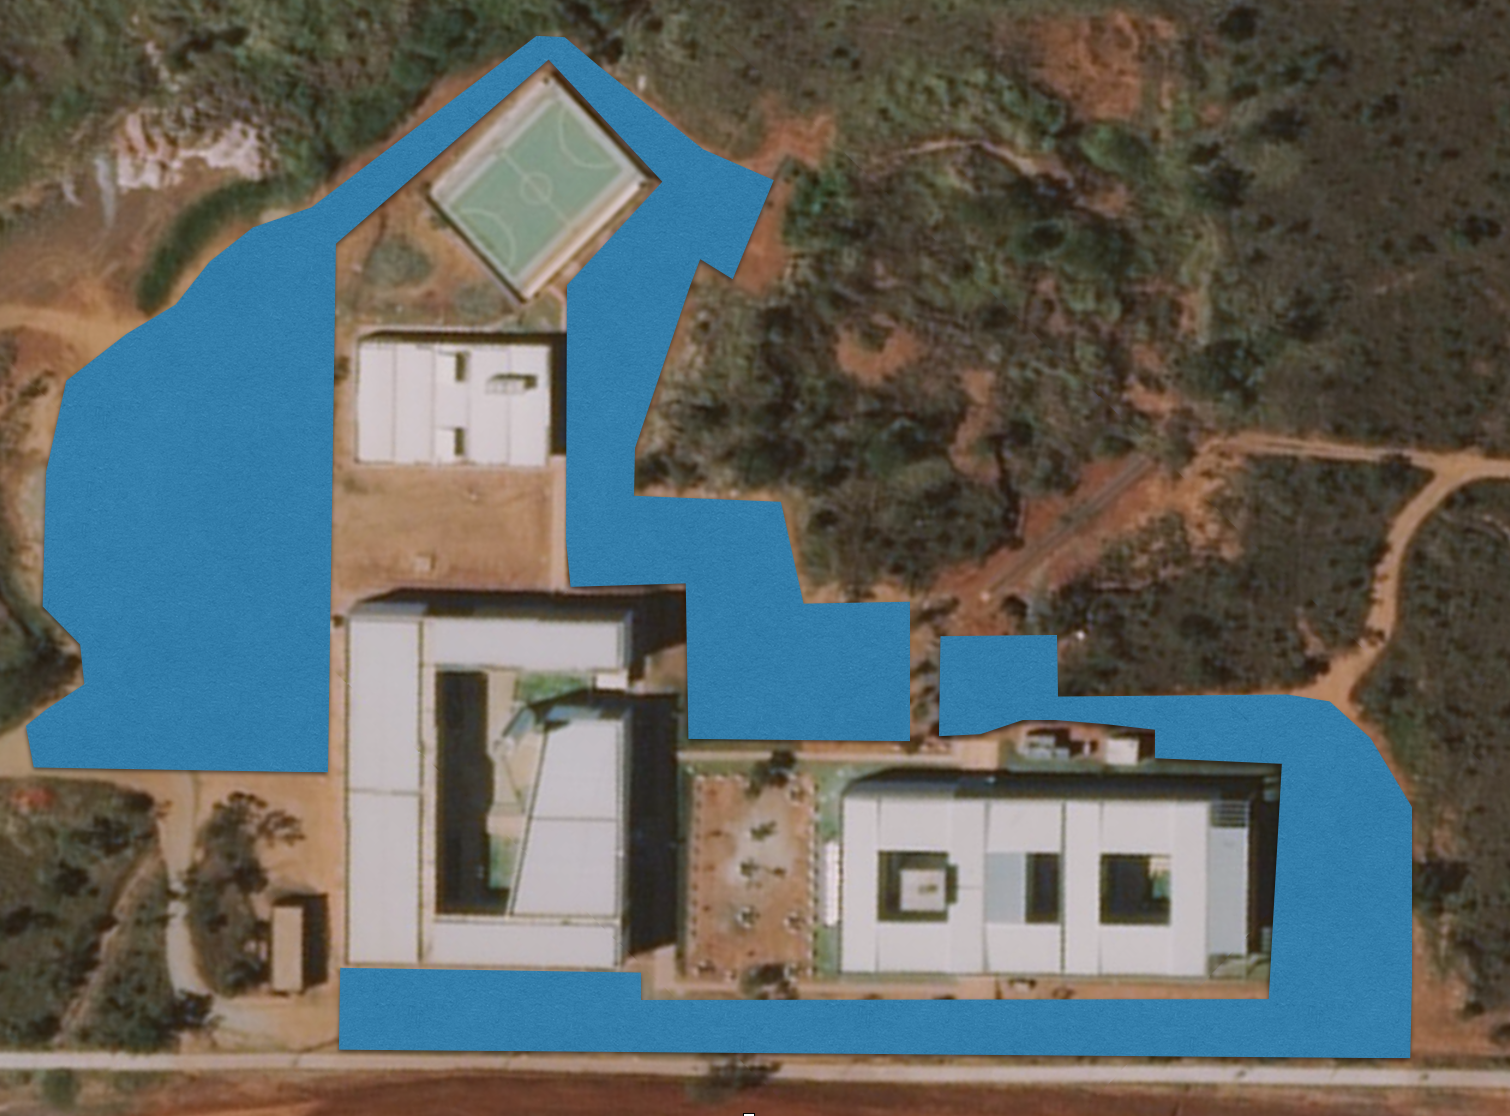
\includegraphics[width=0.87\textwidth]{figuras/fga2}
  \caption{Vista aérea do Campus FGA: áreas de estacionamento do campus.}
  \label{img:fga2}
\end{figure}

Dessa forma, devido à impossibilidade de localizar apenas um balão que possa monitorar todas as áreas de estacionamento, três balões cativos serão posicionados estrategicamente para que o objetivo seja cumprido [figura \ref{img:fga3}].

\begin{figure}[H]
  \centering
  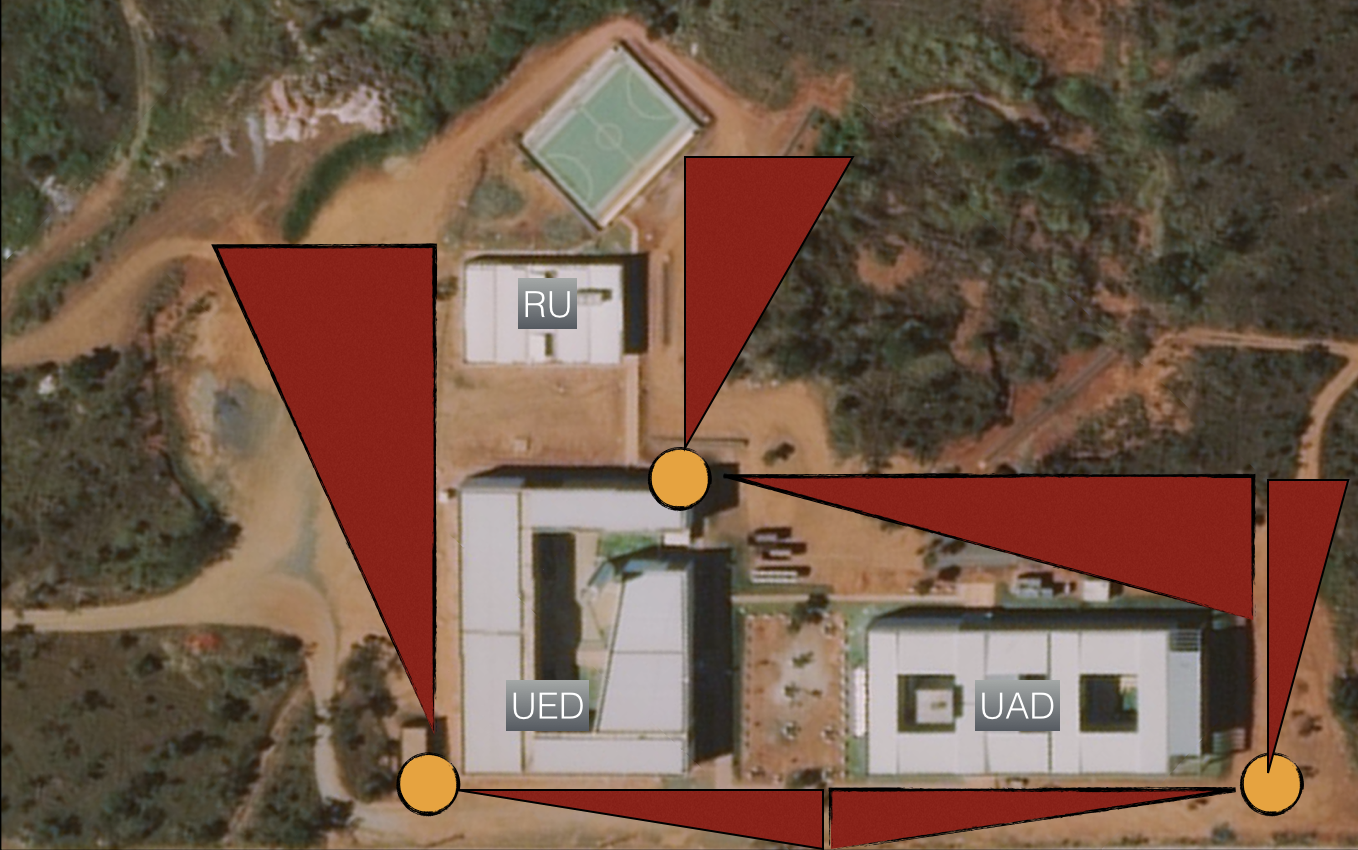
\includegraphics[width=0.87\textwidth]{figuras/fga3}
  \caption{Vista aérea do Campus FGA: áreas de alcance de monitoramento.}
  \label{img:fga3}
\end{figure}



  %\subsection{SUM E A SEGURANÇA DO CAMPUS}
  %\subsubsection{ÁREAS DE MONITORAMENTO}
%\subsubsection{RECONHECIMENTO DE SITUAÇÕES DE RISCO}

    Após coletar informações sobre o modo de operação dos indivíduos responsáveis pelo furto dos carros, foi observado que o mesmo ocorre em um intervalo de tempo variável, mas curto, mesmo em locais movimentados o furto não costuma demorar mais que três minutos em locais sem fluxo de pessoas um bandido experiente consegue realizar o arrombamento e  fugir utilizando o carro roubado em cerca de 30 segundos, em algumas ocasiões, os meliantes gastam mais tempo para escolher o carro que será furtado do que com a ação de verdade. Isso nos fez pensar que o sistema teria que identificar uma situação de risco de forma rápida.
    
    Sendo assim, a partir de análises de mercado, obtivemos os seguintes sistemas de segurança:
    
    \bullet Sistemas gerenciadores de câmeras: Os sistemas gerenciadores de câmeras apenas gravam imagens obtidas através de várias câmeras e disponibilizam essas imagens em um circuito fechado de televisão (CFTV), normalmente, existe um operador de CFTV que é uma pessoa que observa todas as imagens gravadas em tempo real e toma as decisões necessárias quando as situações não desejadas se apresentam.
    
    \bullet Sistemas de segurança inteligente: O sistema de segurança inteligente utiliza diversos sensores para tentar perceber quando algo esta fora do esperado e contactar o administrador do sistema, por exemplo, alguns sistemas inteligentes(S.I.s) utilizam detectores de movimento em suas câmeras para que quando for detectado um movimento isso gere um alarme, outros sistemas utilizam sensores de abertura e assim que este sensor for ativado o alerta seja gerado e enviado, o envio pode se dar de diversas formas, seja o envio de e-mail, ligação, mensagem SMS ou ainda uma notificação de um aplicativo para smartphone.Sistemas inteligentes tem muito a oferecer, visto que, quebrada a barreira de ensinar a máquina a forma de reconhecer alguma situação e como lidar com ela, a possibilidade da máquina falhar em reconhecer e alertar sobre a situação é menor do que a de um ser humano falhar, visto que este esta exposto a uma lista de variáveis que o inclinam em direção ao erro muito maior do que a máquina.A afirmação dada no parágrafo acima pode ser testada ao se comparar a efetividade de um sistema gerenciador de câmeras e um sistema inteligente gerenciador de câmera.

  \bullet Reconhecimento de pessoas: O sistema de reconhecimento de pessoas age por reconhecimento de padrões, seja ele o da voz ou um padrão biométrico, ambos podem ser utilizados em prol da segurança. Pensando em um ambiente externo, onde apenas em raras situações o áudio coletado seria bom e confiável o suficiente para se realizar o reconhecimento, nos resta a opção de padrões biométricos, o que é uma boa opção, afinal, já existem APIs livres para uso e eficientes que prestam esse tipo de serviço, sejam exemplos, a FACE API disponibilizada para desenvolvedores, pela Google inc., em 2015 que consegue identificar pessoas mesmo que estas estejam com o rosto com inclinações diferentes da usual enquanto usa um smartphone, também é capaz de reconhecer as pessoas enquanto estas sorriem ou fecham seus olhos, pois a API calcula a posição onde os componentes do rosto da pessoa estariam e dessa forma consegue realizar a comparação. Outro exemplo foi disponibilizado logo no início de 2015 pelo laboratório de inteligência artificial do Facebook, a API liberada pelo Facebook acelera a velocidade em que a máquina aprende em até 23 vezes o normal e por isso mesmo consegue reduzir os custos consideravelmente.


    De posse destas informações, o grupo entendeu que a melhor solução está em utilizar estas tecnologias para criar uma solução própria, pois nenhuma delas parece completa e segura quando se analisamos os pontos fortes e fracos das três conjuntamente. No entanto, a união dos três tipos de sistema, somado a criptografia, que embora não citada, está presente em qualquer sistema de segurança respeitável, podem formar uma estrutura bem robusta de segurança e bem adaptada para o objetivo do nosso projeto. E isso será mostrado a seguir.
    
    O sistema que tratará as imagens realizará reconhecimento facial para associar o rosto do motorista ao carro em que ele chegou, e quando o sistema identificar uma situação em que uma pessoa não associada a determinado carro está muito próxima ao carro por mais de quatro segundos, ele gerará um alerta. Para que não ocorra um elevado numero de falsos positivos o sistema também executa um  mapeamento das pessoas próximas ao estacionamento e assim prevê o caminho que determinada pessoa pode fazer até chegar ao seu carro e caso essa pessoa permanece próxima a um carro diferente do qual está associada por mais de quatro segundos, mas dentro de um dos caminhos previstos pelo software até seu carro o alerta não será gerado. Por conta da velocidade com que ocorre a consumação do furto, é importante que, sempre que o sistema não conseguir reconhecer algum rosto porque a pessoa intencionalmente cobriu o rosto com algo, seja gerado um alarme independente da proximidade com qualquer veículo.

    \paragraph{Administração}
    \bullet  O sistema possui ferramenta de configurações globais de câmeras, onde o administrador pode aplicar a mesma configuração para um grupo de câmeras ao mesmo tempo.
    \bullet Possui calculadora de disco para calcular o espaço em disco necessário para gravação baseando-se em dados como Resolução, quadros por segundo, tempo desejado para armazenar e estimativa de detecção de movimento.
    \bullet Trabalha com conceito de grupos de alerta onde na ocorrência de um determinado evento, apenas o grupo configurado para receber o alerta será notificado.
    \bullet Possui log de eventos do sistema que registrará todas as atividades dos usuários bem como as atividades do próprio sistema.
    \bullet Possui servidor web embutido no sistema para monitoramento ao vivo e reprodução de vídeo remoto.
    \bullet  Possui suporte a HTTPS e SSL.
    \bullet Fornece ferramenta de monitoramento de desempenho do servidor através de gráficos históricos com informações como: Consumo de processador, consumo de memória, tráfego de entrada em KB/s e tráfego de saída em KB/s.
    \bullet Permite configurar diretório padrão para exportação de mídia e fotos de tela de monitoramento.
    \bullet Busca automática de câmeras na rede através de protocolo UPnP.
    \bullet Permite a localização automática de câmeras que utilizam protocolo ONVIF.
    \bullet O software possibilita a exportação de registros de auditoria e os registros de pesquisas de eventos
    \bullet O sistema pode fornecer o tempo de desconexão de cada câmera
    \bullet Acesso aos logs de eventos pode ser feito somente pelo administrador do sistema ou por usuário por ele autorizado.
    \bullet Possibilita a exportação de relatórios e gráficos do sistema nos formatos PDF
    \bullet Permite pesquisas por data e hora inicial e final, no sistema de auditoria.
    \bullet  Permite que, ao clicar duas vezes sobre um registro de auditoria, este possa ser expandido mostrando todos os seus detalhes.
    \bullet Possui recurso de máscara de privacidade (Inibe determinadas áreas da tela para que seja ocultado algum detalhe da imagem para o operador) para câmeras fixas.
    \bullet Possui filtros para controle da imagem (Blur, Gaussian Blur, Sharpen, Emboss, Flip, Flop, Grayscale e Invert) por câmera (Reprodução de vídeo e Monitoramento ao Vivo) com configurações pré-definidas.
    \bullet O sistema oferece a opção de corte de imagens ( CROP ) com a finalidade de selecionar uma área da imagem que se deseja manter visível para os usuários.
    
    \paragraph{Monitoramento ao Vivo}
    \bullet Suporta monitoramento ao vivo de 6 câmeras.
    \bullet Controle de Matriz Virtual através de SDK/API para criação de macros e scripts em outras linguagens.
    \bullet Sistema de sequenciamento de câmeras, onde o sistema troca automaticamente um grupo de câmeras em tela por outro grupo, também permite a troca manual no sequenciamento.
    \bullet Possui mosaico automatizado de modo que o sistema deverá ajustar o formato de visualização da tela automaticamente, dependendo do número de câmeras em tela.
    \bullet Permite que os mosaicos de monitoramento sejam atualizados dinamicamente em tempo real quando criados, atualizados ou apagados, sem a necessidade de reconexão com o servidor.
    \bullet Permite aumentar a taxa de quadros de uma determinada câmera no monitoramento, quando selecionada (Ex: Monitoramento normal em 4FPS, se o usuário selecionar a câmera, aumentar para 30FPS, quando o usuário deselecionar a câmera, sua taxa de quadros deve retornar para 4FPS).
    \bullet Possui detecção de movimento em tempo real no monitoramento ao vivo. Esta função faz com que o movimento seja marcado com uma cor específica na tela.
    \bullet Permite que operações remotas possam fazer uma gravação local de emergência, gravando assim as imagens que estão sendo monitoradas.
    \bullet No monitoramento ao vivo, é possível fazer o zoom (Digital) de diferentes partes da tela, abrindo assim uma tela para cada zoom digital realizado.
    \bullet Possui sistema de zoom com tratamento bilinear para evitar que a imagem fique quadriculada. Suporta dois ou mais monitores de vídeo por estação para o monitoramento ao vivo.
    \bullet Clique em uma câmera para selecioná-la e maximizá-la. Opção de remover câmera da tela. Possibilita informações das câmeras como resolução da imagem, Frames por segundo "FPS", Taxa de Transferência e Decoder.
    \bullet Identificação automática na tela, o status de funcionamento das câmeras através de diferentes ícones da lista de objetos, ex: câmera gravando por movimento, por evento, por evento e movimento, parada, em funcionamento, etc.. Sistema de Segurança Digital Descritivo de recursos do sistema
    \bullet Exibe informações sobre as câmeras, informando através de indicadores visuais o status do dispositivo.
    \bullet Permite abrir as câmeras clicando diretamente no seu ícone do mapa.

  \subsubsection{PARCERIA SEGURANÇA DO CAMPUS E SUM}
    O reconhecimento de situações de risco por si só não geraria os resultados esperados, pois o software não tem a capacidade de julgar uma ação como criminosa ou como um incidente comum. Visto isto, decidiu-se realizar uma integração entre o sistema automatizado e os seguranças da faculdade.
    
    Esta parceria aconteceria da seguinte maneira: o sistema realizaria todas as ações repetitivas da segurança, como vigiar os carros, identificar os responsáveis do veículo, só que de maneira automatizada. Porém, este sistema não conseguiria ter plena certeza que ao identificar uma possível ação criminosa estaria de fato ocorrendo uma. Para evitar que a polícia fosse chamada a cada possível crime, o sistema emitiria alertas através de ligações telefônicas quando julgasse uma situação de risco, através de uma mensagem gravada indicaria o local do ocorrido para que os seguranças fossem averiguar a natureza do alerta e tomarem as devidas providências, se necessário.
    
    \paragraph{Alertas e Eventos}
    O sistema possui um completo gerenciamento de alarmes e eventos, com reconhecimento de alarmes de qualquer dispositivo. Este gerenciamento de alarmes contempla as seguintes funcionalidades:
    
    \bullet Na ocorrência de um alarme externo, no caso em algum dos carros, o sistema tomará ações proativas para alertar os operadores, como exemplo, janelas de alerta com áudio para chamar a atenção.
    \bullet Todas estas ações de alarme podem ser configuradas independentemente para cada câmera e todas devem ter um agendamento de operação, sendo que apenas serão chamadas se o agendamento permitir.
    \bullet O Sistema toma ações proativas na detecção de movimento das câmeras em horários pré-definidos, ou seja, se em determinado horário que não pode haver movimento em determinada câmera o sistema reconhecer um movimento, então este poderá tomar ações de alarme.
    \bullet  O Sistema também poderá tomar todas estas mesmas ações proativas caso a câmera ou servidor de vídeo venha a ficar fora de funcionamento e / ou ocorrer algum erro na gravação das imagens.
    \bullet  Fornece ações de alarme manual, onde o operador poderá através de um clique em uma lista de ações, disparar as ações proativas.
    \bullet O Sistema fornece um agendamento de reconhecimento de alarmes externos por câmera, ou seja, tem a possibilidade de reconhecer os alarmes apenas em horários específicos. Sistema de Segurança Digital Descritivo de recursos do sistema.
    \bullet Tem a capacidade de gravar as imagens na ocorrência de um evento e também fornecer um agendamento de transmissão de imagens onde possibilita a transmissão dessas imagens apenas na ocorrência de um alarme.
    \bullet Permite que com o acionamento do alarme de uma câmera possa-se iniciar a gravação e/ou transmissão de imagens de quaisquer outras câmeras.
    \bullet Diversos sons de alarme para que os operadores possam diferenciar cada alarme através de um som diferente.
    \bullet Permite o agendamento de um ou mais eventos para que eles ocorram em qualquer dia do mês e ano desejado.
    \bullet  Permite pesquisar no banco de dados de eventos, através do tipo de evento, filtro por datas, objetos e outros, as ocorrências internas e externas ao software, relacionadas aos alarmes do sistema.
    \bullet Permite que no sistema de análise de imagens, os objetos que estiverem alarmados por alguma regra de analítico tenham o seu contorno alterado para uma determinada cor, por exemplo vermelho.
    \bullet Permite evento de detecção de áudio caso o nível esteja acima ou abaixo de um limite especificado por um tempo determinado.
    \bullet Permite gerar evento de falha de comunicação se o dispositivo permanecer fora de funcionamento por mais de X segundos, com opção de continuar gerando o evento a cada X segundos enquanto o dispositivo estiver off-line.
    \bullet Permite detecção de nível de áudio para alertas e eventos.
  
\subsection{ESTRUTURA SUM}

   A estrutura do balão será dividida em três partes principais: a bexiga, local onde será armazenado o gás; payload, que será o local de armazenamento dos equipamentos eletrônicos; elevador, que consite o cabo preso ao payload do balão e também o sistema eletromecânico em solo que libera o fio (elevando o balão) ou retrai o fio (desce o balão).

\subsection{Payload}
  
    A estrutura da payload foi inspirada em um padrão de nanosatélites 9U, figura \ref{img:payload}, porém com adaptações. A estrutura de um CubeSat 1U possui as dimensões deste são de um cubo 10 x 10 x 10 cm, ou seja, o termo 1U diz respeito as dimensões do sistema. Dessa forma um 9U significa que suas dimensões são 30 x 30 x 10 cm, e colocando de outra forma, é equivalente à três nanosatélites 3U em conjunto. A parte superior será acoplada à bexiga, enquanto que a inferior, ao cabo.

  \begin{figure}[H]
    \centering
    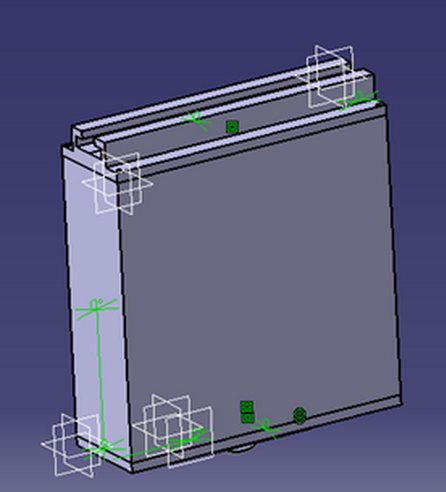
\includegraphics[width=0.5\textwidth]{figuras/payload}
    \caption{Representação da estrutura da payload. }
    \label{img:payload}
  \end{figure}


    Segundo Yajima, existem três tipos de sistemas de balões que são utilizados: balão zero pressão, balão super-pressão e uma combinação entre os dois sistemas. O sistema mais adequado à aplicação proposta mostrou-se o balão zero pressão.Existem vários modelos de balão: esférico, cilíndrico, tetraédrico e formato natural. O modelo utilizado será o modelo de balão esférico, pois esse modelo é o que apresenta menos complicações nos cálculos de dimensionamento de volume, empuxo, gás e etc.

    O gás que será utilizado no balão será o Hélio, este gás possui algumas desvantagens em relação ao gás Hidrogênio[2], que é mais leve, porém por ser um gás inerte o Hélio é a principal opção  de uso[3]. Ficou decidido que a massa  máxima  da payload será de 20 kg.

    O material usado para a confecção da bexiga será a Aramida (Kevlar), pois  esse material apresenta propriedades mecânicas interessantes, como elevada tenacidade, baixo alongamento e resistência ao calor[10],  além de ser considerado um material leve[8]. Com esses dados em mãos foi possível calcular o raio mínimo que o balão deveria ter, o valor foi de 2 metros. Para uma margem de segurança será adotado um valor de raio do balão entre 2 metros e 2,5 metros. As forças de empuxo e peso do balão variam de acordo com o raio. O empuxo com o raio igual a 2 metros é de cerca de 403N, com o raio igual a 2,5 metros o empuxo é de 786N, será avaliado o material utilizado na ancoragem do balão,  e dependendo da resistencia à tração desse material será adotado um raio fixo para o balão.

\subsection{Funcionamento}
    O horário de funcionamento do balão será das 6h às 21h, o sistema ficará a uma altura entre 30 metros e 50 metros para uma melhor visualização do movimento do estacionamento.

    O estudo das condições ambientais e o dimensionamento dessas variáveis são fundamentais para a estabilidade do balão. A força de arrasto no balão devido a um vento de 12m/s, na pior das hióteses, seria na ordem de 3,8kN.

  \subsubsection{Sistema do Balão}
    Das opções para o sistema do Balão existem três opções: Balão Pressão Zero, Balão Super-Pressão e uma combinação dos 2 sistemas.
    O sistema escolhido para o balão foi o sistema de pressão zero. Os fatores que nos levaram a escolha desse sistema é sua capacidade de regular sua altitude, seu modo de funcionamento que facilita a descida do balão após o horário de funcionamento e a fácil implementação, ao contrario do balão super pressão que exige que a espessura do envelope do balão seja bastante alta, em alguns casos a pressão suportada por um balão de super pressão é varios fatores de 10 maior que a pressão suportada por um balão de pressão zero.

    O Balão Pressão Zero é assim denominado pelo fato da diferença de entre a pressão interna ao envelope do balão e a pressão externa ser zero na base do balão, local onde o balão é conectado a atmosfera por um duto de ventilação.
    
    O duto funciona de tal modo que quando a pressão interna na base do balão excede a pressão da atmosfera exterior o duto é empurrado para fora e forma uma um cilindro que permite que parte do gás seja expelida. Quando a diferença de pressão é negativa, a pressão atmosferica empurra o duto para dentro, impedindo a entrada de ar.
    
    Após atingir sua condição de completamente inflado ele ascende até a posição em qua a força de flutuabilidade se iguala ao seu peso. Essencialmente a temperatura do gás de sustentação durante a ascensão é inferior a da atmosfera, em decorrencia do efeito da expansão adiabática. Quando a ascensão termina a temperatura do balão se iguala a da atmosfera isto compensará a redução da sustentação devido a ventilação excessiva.
    
    Uma caracteristica importante dos Balões Pressão Zero é o assim chama, efeito do ocaso. Como o balão tem uma altitude de estabilidade apenas quando ascende, após o por do sol o balão para de absorver radiação do sol, a temperatura do gás de sustentação cai, e consequentemente, a  força de flutuabilidade o que faz o balão nãomander sua altitude.
    
    Já que o periodo de funcionamento do Balão se dará entre 6h da manhã e as 21h a queda de altitude da noite é interessante  para a logistica, já que após esse horário o balão é recolhido.
    
\begin{table}[h]
\caption{Características do Hélio}
\vspace{0.5cm}
\begin{tabular}{|r||lr}
\hline

Calor latente de fusão a 1,2 K, 2555 kPa & 0,3347 J/mol; 0,08cal/mol.\\
Calor molar específico, gás a 101,325 kPa a 25ºC a pressão constante & 20,967 J/(mol x K) \\ 
Calor molar específico, gás a 101,325 kPa a 25ºC a volume constante  & 12,863 J/(mol x K)                                       \\
Condutividade térmica, gás a 101,325 kPa a 26,85ºC                   & 0,017744 W/(m x K); 0,425 x 10-6 cal x cm/(s x cm2 x ºC) \\
Densidade absoluta, gás a 101,325kPa a 0ºC.                          & 0,1785 Kg/m3                                             \\
Densidade crítica                                                    & 0,5307 Kg/dm3                                            \\
Densidade relativa, gás a 101,325 kPa a 0ºC,(ar = 1).                & 0,138                                                    \\
Fator crítico de compressibilidade                                   & 0,305                                                    \\
Fórmula                                                              & H^4e                                                      \\
Massa Molecular                                                      & 4,002602                                                 \\
Pressão crítica                                                      & 229 kPa ; 2,29 bar; 33,2 psia;,2,261 atm.                \\
Solubilidade em água a 101,325 kPa (pressão,parcial),a 20ºC          & 8,61 cm3 /1 Kg de água                                   \\
Temperatura crítica                                                  & 5,20 K; -268ºC; -450,3ºF                                 \\
Viscosidade, gás a 101,325 kPa a 26,8ºC.                             & 0,02012 mPa x s; 0,02012 cP.                             \\
Volume crítico                                                       & 14,431 dm3/ kg                                           \\
Volume específico a 21,1ºC 101,325 kPa                               & 0,017744 W/(m x K); 0,425 x 10-6 cal x cm/(s x cm2 x ºC)
\hline
\end{tabular}
\end{table}

\begin{table}[h]
\caption{Características do Hidrogênio.}
\vspace{0.5cm}
\begin{tabular}{|r|lr}
\hline

Calor molar específico, gás a 101,325 kPa a 
 26,8ºC a pressão constante &  28,851 J/(mol x K)\\
Condutividade térmica, gás a 101,325 kPa a 
 26,8 ºC. & 0,181699 W/(m x K);
 434,3 x 10-6 cal/(s x cm x ºC) \\ 
Densidade absoluta, gás a 101,325 kPa a 25ºC  & 0,08235 kg/m3 \\
Densidade crítica   & 0,0310 kg/dm3 \\
Densidade relativa, normal, gás a 101,325 kPa
 a 25ºC (ar=1) &  0,0695\\
Fator crítico de compressibilidade & 0,305 \\
Fórmula   & H_2 \\
 Limites de inflamabilidade no ar & 4,0-75\% (por volume)\\
Massa Molecular & 2,01588 \\
Pressão crítica  & 1297 kPa; 12,97 bar; 188,1 psia;  12,80 atm \\
Temperatura de auto-ignição & 844,3 K; 571,2ºC; 1060ºF\\
Viscosidade gás a 101,325 kPa a 26,8ºC  & 0,008957 mPa x s; 0,008957 cP\\
Volume específico a 21,1ºC, 101,325kPa & 11967,4dm3/kg; 191,7ft3/lb\\

\hline
\end{tabular}
\end{table}

    O gás hidrogênio a primeira vista é mais vantajoso pois é mais leve que o hélio, sua densidade relativa é de 0.0695 enquanto que a do hélio é de 0.138, e apresentam um fator crítico de compressibilidade iguais. Porém o hidrogênio possui a característica de ser inflamável, enquanto que o hélio é conhecido por ser um gás inerte. Tendo em vista a segurança dos usuários do estacionamento e dos funcionário responsáveis pela manutenção do balão, a exposição ao sol e a possíveis, porém improváveis,  descargas elétricas o hélio se mostra a opção mais vantajosa.
    
    \subsubsection{Forças no Balão}
    As principais forças que atuaram no Balão serão o peso do balão e sistemas integrados, a força de sustentação provocada pelo gás e a forças externas provocadas pelo vento relativo. O peso do balão e a sustentação foram calculados a partir de uma estimativa da massa total do balão e a faixa de altitude onde ele irá atuar. As forças relativas as condições de vento foram calculadas a partir da análise das condições climáticas do Distrito Federal.
    
    Os dados climáticos foram colhidos a partir do Banco de Dados Meteorológicos disponibilizado pelo Instituto Nacional de Meteorologia (INMET) em seu site durante o Período de 01/01/2005 até 31/12/2014.
    
    \paragraph{Preliminar análise de estabilidade dinâmica do balão cativos}
    Um dos problemas em balões cativos é definir a sua configuração de equilíbrio. Durante o vôo, o balão está sujeito a perturbações atmosféricas, principalmente devido a variação da velocidade do vento, essas perturbações podem levar instabilidade ao balão.
    
    Para um aero-monitoramento é crítico que as câmeras sejam capazes de obter imagens em alta qualidade, portanto o sistema precisa estar o mais estável possível.
    
    %CONTINUAR APÓS DESCOBRIR COMO COLOCAR IMAGENS!
  %\subsection{SUM E A CAPTAÇÃO DE IMAGENS}
  %\subsubsection{POSICIONAMENTO DE CÂMERAS}
  %\subsubsection{SISTEMA DE CAPTAÇÃO DE IMAGENS  E CONDIÇÕES CLIMÁTICAS}
  
  %\subsection{SUM E A ESTAÇÃO DE SOLO}
  %\subsubsection{ENVIO DE DADOS}
  %\subsubsection{RECEBIMENTO DE DADOS}
  %\subsubsection{DINÂMICA DE OPERAÇÃO DE DADOS}
  
  %\subsection{SUM E HORÁRIO DE FUNCIONAMENTO}
  %\subsubsection{DIAS DE FUNCIONAMENTO}
  %\subsubsection{RECOLHIMENTO DO BALÃO}
  
\subsection{SUM E ALIMENTAÇÃO}

  \subsubsection{Tipos de Alimentação}
Para a alimentação do aeróstato de monitoramento do estacionamento da Faculdade do Gama foram consideradas três possibilidades: energia solar, eólica e a cabo.  Contudo, é preciso analisar, de maneira objetiva e realista, a opção que melhor  atende às demandas de seu funcionamento, ao ambiente no qual o balão estará localizado e à viabilidade econômica de sua manutenção.

Dessa forma, necessita-se de uma avaliação concisa das três opções disponíveis, abrangendo sua eficiência, operacionabilidade, custos e manutenção, respectivamente.
  
  \subsubsection{Energia Solar}
  Painéis solares fotovoltáicos, são dispositivos usualmente utilizados para conversão de energia proveniente do sol, em energia elétrica. Estruturalmente, painéis solares são compostos por células solares, capazes de criar uma DDP (Diferença de Potencial) através do fluxo de corrente elétrica.
    
    \paragraph{Eficiência}
  Eficiência é atingir o resultado com o mínimo de perdas de recurso, e quando falamos em uma placa fotovoltáica, falamos na quantidade de energia recebida, convertida em energia elétrica disponível para utilização. Em um painel solar, quanto maior a produção energética por metro quadrado de placa, melhor a eficiência do sistema. Atualmente, a média de valores referente à eficiência dos painéis solares comerciais fica entre 14\% e 21\%.
    
    \paragraph{Operacionabilidade}
  Inicialmente, devemos analisar o consumo energético,em kWh, que será demandado pelo aeróstato cativo, com base nisso, é feito o dimensionamento do sistema de geração.
    
  Após a estimativa de consumo, o próximo passo é a instalação dos painéis solares, levando em conta o direcionamento, inclinação, posição geográfica e incidência solar mensal. Para isso, existem softwares os quais auxiliam no processo de apontamento, aumentando a eficiência do sistema.
    
  Finalizando todas as etapas de dimensionamento, instalação, apontamento e análise dos dados de geração, o processo pode ser considerado simples, e de baixa complexidade de opreação para pequenos sistemas.
    
    \paragraph{Custos}
  Os custos iniciais de implantação de um sistema solar no Brasil, ainda é muito caro, devido a maior parte dos componentes serem importados e taxados com impostos e a opção começa a se tornar pouco atraente quando levamos em conta sua eficiência e comparamos com outros sistemas de geração.
  
   \paragraph{Manutenção}
  A manutenção dos painéis solares é simples, de baixo custo, e o processo não precisa de mão de obra extremamente especializada. De forma simplificada, a manutenção do painel consiste na limpeza das superfícies, uma verificação do cabeamento, e correções no apontamento de tempos em tempos.
  
\subsubsection{Energia Eólica}
  Devido a sua característica inesgotável e não poluidora, sendo, portanto, uma fonte de energia renovável, a energia eólica vem tomando espaço no estudo sobre aerogeradores \cite{rocha2010}. Segundo \cite{Evans20091082}, é um sistema que com menor emissão de CO2, com apenas 25 g/kW h CO2-e.
  
  \paragraph{Eficiência}
  Segundo \cite{Evans20091082}, a eficiência energética da energia eólica está entre 24-54\%.
  
  \paragraph{Operacionabilidade}
  O modelo de aerogerador poderá apresentar eixo horizontal, com rotor em forma de balão de hélio, com transmissão de força para baixo pelo auxílio de cabos, bem como é apresentado no projeto da empresa Magenn Air Rotor System (MARS) \cite{texeira2012}.
  
  Podendo as turbinas sofrerem intermitência, \cite{edmondes2007}. propõe uma capacidade distribuída sobre uma ampla área, aliviando as flutuações. As turbinas não podem operar quando a velocidade do vento é muito alta (>25 m/s), pelo fato de que danos na turbina podem ocorrer e estas não poderão funcionar quando a velocidade do vento estiver muito baixa (< 3 m/s) (WEC, 2007).
  
  \paragraph{Custos}
  Mesmo se tratando de uma fonte de energia limpa, os custos de instalação de tecnologias para geração de energia elétrica são muito altos. Principalmente no Brasil, tendo em vista que o custo elevado pode se dar aos custos logísticos de implantação do projeto, como o número restrito de ofertantes nacionais também associado às restrições de importação de aerogeradores.
  
  A oferta de turbinas eólicas no Brasil se restringe apenas a duas firmas que possuem suas vantagens, entre elas: imposto de 14\% sobre a importação de aerogeradores, sendo que apenas aqueles que possuem potência superior a 1,5 MW que poderão ser importados e o BNDES só concede financiamento aos fabricantes nacionais.

  O custo de manutenção para turbinas no inicio de sua vida útil normalmente é mais baixo quando comparado com o custo para turbinas que tenham maior tempo de funcionamento. Para máquinas novas, é estimado um custo anual de 1,5 a 2\% do investimento, enquanto para turbinas com maior tempo de funcionamento o custo do investimento sai em torno de 3\% ao ano.
  
  \paragraph{Manutenção}
  Os sistemas eólicos necessitam de pouca manutenção. A vida útil de suas turbinas eólicas é de 15 anos, e os dispositivos eletrônicos, como inversor e controlador de carga, são avaliados em 10 anos. Já os sistemas eólicos isolados com o armazenamento de energia em baterias, as quais são consideradas o ponto crítico do sistema, que quando bem projetado poderá ter uma vida útil de 4 a 5 anos.

  \subsubsection{ENERGIA ON GRID}
  Um sistema ligado on grid, é aquele que trabalha em conjunto com a rede elétrica que é fornecida pela concessionária responsável pela distribuição energética na região.

    \paragraph{Eficiência}
    A eficiência de um sistema de transmissão, é um fator altamente importante no processo, já que ele é o responsável pela economia dos custos. Existem fatores diretamente ligados nos custos da produção energética, como grandes períodos de estiagem, local de geração, e matriz energética. O planejamento visa sempre o menor custo, e o objetivo é sempre atingir a menor perda possível no processo de geração e transmissão.  Para isso, usamos tensões muito elevadas,  para uma potência elétrica igual, assim, tendo uma menor corrente elétrica. Como as principais perdas no sistema são térmicas, a lei de Joule, diz que, a perda é diretamente proporcional a corrente elevada ao quadrado, tendo que reduzindo a corrente e aumentando a tensão, a redução nas perdas no processo são reduzidas de forma significante.
    
    \paragraph{Operacionabilidade}
    Inicialmente, devemos saber qual a carga energética que será demandada pelo balão para que o dimensionamento do sistema de alimentação possa ser feito. Informações como demanda energética, períodos de maior consumo, horário de funcionamento, são cruciais para que tenhamos uma otimização dos insumos energéticos, diminuindo assim, os custos de operação do balão. A gestão energética do balão é feita por um quadro de distribuição de energia com indicatores de tensão, corrente e consumo instantâneo, para que seja monitorado se as condições mínimas condições de funcionamento estão sendo atendidas. A transmissão da energia para o balão será feita via cabo, devidamente dimensionado à uma bitola compatível, de material flexível, e leve, que não afete a mobilidade do balão.

    \paragraph{Custos}
    Os custos desse tipo de transmissão de energia estão relacionados a tecnologia de transmissão e ao equipamento que está sendo ligado na rede. Além desses custos, que estão diretamente ligados aos componentes físicos do sistema, existem tributos e encargos cobrados na conta de energia elétrica.
    
    De acordo com a Agência Nacional de Energia Elétrica, a ANEEL, a soma dos encargos tributários na conta de luz atualmente podem chegar a 45\%. A variação da tributação do kWh, varia de acordo com o consumo de energia.
    
    Os custos são contabilizados pelo quadro de distribuição energética instalado no recebimento da rede, o qual contabiliza quantos Watts foram utilizados em um determinado período de tempo, gerando um conta referente ao consumo, que deve ser paga à concessionária fornecedora de energia.

  \paragraph{Manutensão}
  A manutenção de um sistema de alimentação on grid, pode ser dividido em duas etapas, a primeira, após o quadro de distribuição, que fica de responsabilidade do proprietário do sistema, cuidar da integridade dos cabos e dimensionamento do conjunto, e a segunda, antes do quadro de distribuição, que fica de responsabilidade da concessionária fornecedora de energia elétrica da região, tendo obrigação de cuidar do fornecimento, integridade e constância da alimentação da rede.
